%%%%%%%%%%%%%%%%%%%%%%%%%%%%%%%%%%%%%%%%%%%%
%%%%%%%%%%%%%%%%%%%%%%%%%%%%%%%%%%%%%%%%%%%%
% Import preamble
\documentclass[aspectratio=169,xcolor=dvipsnames, 11pt]{beamer} 

%\documentclass[xcolor=dvipsnames,mathserif]{beamer} % this option has curvier math
%\documentclass[xcolor=dvipsnames,11pt]{beamer}
% Note: the color structure needs to be added here in the title. Now it recognizes all beamer % colors.

%%%%%%%%  PRESENTATION LAYOUT:
\usepackage{appendixnumberbeamer} % this package does not count the appendix pages.
\mode<presentation>
{
  \usetheme{Boadilla}
  \usecolortheme{lily} % lily is nice or orchid but not for definition
  \setbeamercovered{invisible}
  \setbeamertemplate{footline}{\raggedleft\insertframenumber~/~\inserttotalframenumber\hspace*{3pt}\vskip3pt} %this command shows frame number, not page number at bottom (means if using overlays, % frame number does not change)
%\setbeamertemplate{footline}[page number]  % this puts only page number on bottom
 \setbeamertemplate{navigation symbols}{}  % this erases navigation symbols.
 \setbeamersize{text margin left=0.2cm, text margin right=0.1cm}
 \setbeamertemplate{frametitle}[default][center]
 \setbeamercolor{frametitle}{fg=black}
 \setbeamerfont{frametitle}{size=\large, series=\bfseries} % Modifies frame title font.
 \setbeamercolor{button}{fg=blue, bg=white}
 \setbeamertemplate{itemize item}[circle]
 \setbeamercolor{itemize item}{fg=black}
 \setbeamercolor{itemize/enumerate body}{fg=black}
 \setbeamerfont{framesubtitle}{series=\mdseries}

}

\renewcommand{\familydefault}{\rmdefault} %Options here are \ttdefault \ssdefault or \rmdefault.

% This defines actual color palette; 
\definecolor{blue}{RGB}{0,114,178}
\definecolor{red}{RGB}{213,94,0}
\definecolor{yellow}{RGB}{240,228,66}
\definecolor{green}{RGB}{0,158,115}
\definecolor{orange}{RGB}{230,159,0}

\hypersetup{
  colorlinks = false,
  linkbordercolor = {white},
  linkcolor = {blue}
}

%%% Color customization: where these colors are used. 
\colorlet{cwords}{blue} %this defines a color, stored under the name cwords that will be used and recognized in document.
\colorlet{cwordsc}{red} %color for contrast with some other word.
\colorlet{cwords2}{green} %2nd color for contrast with some other word.
\colorlet{cmath}{blue} %color for math in text.
%\everymath{\color{blue}} % This in conjunction with the everysel package sets color of math
\everydisplay{\color{blue}}


%%%%%%%%  PACKAGES USED:
\usepackage{amsmath}
\usepackage{setspace} % Only needed for spacing
\usepackage{changepage} % Only needed for local margin setting
\usepackage{mathpazo}% font, is overwritten by times
%\usepackage[hypertexnames=false]{hyperref} %This makes hyperref ``dumber'', and, hence, more robust! (otherwise sometimes the appendix links don't work).
\usepackage{hyperref}
\usepackage{multimedia}
\usepackage[english]{babel}
\usepackage{graphicx}
\usepackage{caption}
%\usepackage{subfig}
\usepackage{subfloat}
\usepackage[en-US]{datetime2}
\usepackage{tabulary}
\usepackage{tabularx}
\usepackage{array,booktabs} % Needed for esttab tables according to the "inequality survey."
\newcommand{\sym}[1]{{#1}} % for symbols in Table
\usepackage[T1]{fontenc}
\usepackage[utf8]{inputenc}
\usepackage{times} % This is a different font.
\usepackage[overlay,absolute]{textpos}
%%%\usepackage{animate} % Animate graphs BUG
\setlength{\TPHorizModule}{1cm}
\setlength{\TPVertModule}{1cm}
\captionsetup[figure]{labelformat=empty} % removes caption prefix figure
\setlength{\itemsep}{\fill} % this is supposed to stretch items across full frame.
%\setlength{\parskip}{0.8\baselineskip} % This affects spacing between normal lines (not itemized).
\usepackage{colortbl} % For cell colors
\usepackage[final]{pdfpages}
\usepackage{caption}
\usepackage{subcaption}
%\captionsetup{justification   = raggedright,
%              singlelinecheck = false}
%\usepackage{adjustbox} % to use resizebox for tables size.
\usepackage[export]{adjustbox} % to use resizebox for tables size.
\usepackage{eurosym}
\usepackage{gensymb}

%% TIKZ
\usepackage{tikz}
\usetikzlibrary{er, positioning,decorations.pathmorphing,calc}
\usepackage{tikzscale}

\tikzset{every entity/.style={draw=black, fill=white}}
\tikzset{comment/.style={draw=white, fill=white}}
\tikzset{
	invisible/.style={opacity=0},
	visible on/.style={alt=#1{}{invisible}},
	alt/.code args={<#1>#2#3}{%
		\alt<#1>{\pgfkeysalso{#2}}{\pgfkeysalso{#3}} % \pgfkeysalso doesn't change the path
	},
}

% Commands from template
\newcommand{\alrt}[1]{{\color{alert} #1}}
\newcommand{\alrtl}[1]{{\color{alert}\large #1}}
\newcommand{\alrtL}[1]{{\color{alert}\Large #1}}
\newcommand{\struc}[1]{{\color{structure} #1}}
\newcommand{\strucL}[1]{{\color{structure}\Large #1}}
\newcommand{\strucl}[1]{{\color{structure}\large #1}}
\newcommand{\dred}[1]{{\color{darkred} #1}}
\newcommand{\dredl}[1]{{\color{darkred}\large #1}}
\newcommand{\dredL}[1]{{\color{darkred}\Large #1}}
\newcommand{\altc}[1]{{\color{darkgreen}\textbf{#1}}}
\newcommand{\altcl}[1]{{\color{darkgreen}\textbf{\large #1}}}
\newcommand{\altcL}[1]{{\color{darkgreen}\textbf{\Large #1}}}
\newcommand{\hush}{\hushit}
\newcommand{\hushalrt}[1]{\hushit{{\color{alert} #1}}}
\newcommand{\hushalrtl}[1]{\hushit{{\large\color{alert} #1}}}
\newcommand{\hushalrtL}[1]{\hushit{{\Large\color{alert} #1}}}
\newcommand{\hushstruc}[1]{\hushit{{\color{structure} #1}}}
\newcommand{\hushstrucl}[1]{\hushit{{\large\color{structure} #1}}}
\newcommand{\hushstrucL}[1]{\hushit{{\Large\color{structure} #1}}}


\setbeamertemplate{caption}[numbered]

%%%%%%%%%SECTION TITLES DISPLAYED ON FULL PAGE %%%%%%%%%%
%%%%%%%%%%%%%%%%%%%%%%%%%%%%%%%%%%%%%%%%%%%
\AtBeginSection[]{
  \begin{frame}
  \vfill
  \centering
  \begin{beamercolorbox}[sep=8pt,center,shadow=true,rounded=true]{title}
    \usebeamerfont{title}{\huge \color{red} \insertsectionhead} \par
  \end{beamercolorbox}
  \vfill
  \end{frame}
}

\AtBeginSubsection[]{
  \begin{frame}
  \vfill
  \centering
  \begin{beamercolorbox}[sep=8pt,center,shadow=true,rounded=true]{title}
    \usebeamerfont{title}{\huge \color{blue} \insertsubsectionhead} \par
  \end{beamercolorbox}
  \vfill
  \end{frame}
}

%
% Custom font for a frame.
%
\usepackage{environ}
\newcommand{\customframefont}[1]{
\setbeamertemplate{itemize/enumerate body begin}{#1}
\setbeamertemplate{itemize/enumerate subbody begin}{#1}
}

\NewEnviron{framefont}[1]{
\customframefont{#1} % for itemize/enumerate
{#1 % For the text outside itemize/enumerate
\BODY
}
\customframefont{\normalsize}
}

%%%%%%%%%%%%%%%%%%%%%%%%%%%%%%%%%%%%%%%%%%%%%%%%%%%%%%%
%%%%%% OTHER PIECES OF TEMPLATE FILE
%%%%%% DELETE ONCE CLEAR THAT NOTHING IS MISSING
%%%%%%%%%%%%%%%%%%%%%%%%%%%%%%%%%%%%%%%%%%%%%%%%%%%%%%%


%\documentclass[aspectratio=169]{beamer} % wide
%\usepackage{amsmath,amsthm,fancyhdr,setspace,graphicx,booktabs,pdflscape}
%\usepackage{geometry}
%\usepackage{etex}
%\usepackage{xcolor,colortbl}
%\usepackage{beamerprosper}
%\usepackage{url}
%\usepackage{enumerate}
%\usepackage{graphicx}
%\usepackage{hyperref}
%\usepackage{multicol}
%\usepackage{caption}
%\usepackage{beamerprosper}
%\usepackage{pgfpages, pdfpages}
%\usepackage{tikz-cd}
%
%\usepackage{tabularx}
%\usepackage{anyfontsize}
%\usepackage{multicol,tabto}
%
%\usepackage{float}
%\usepackage{soul}
%\usepackage{grffile}
%\usepackage{changepage}
%\usepackage{sansmathaccent}
%\pdfmapfile{+sansmathaccent.map}
%
%
%\usetikzlibrary{er,positioning,calc,decorations.pathreplacing}
%
%\mode<presentation>
%\usefonttheme{structuresmallcapsserif}
%\setbeamertemplate{footline}[frame number]{}
%\setbeamertemplate{navigation symbols}{}
%
%%change font
%\usefonttheme{default}
%\setbeamertemplate{footline}[frame number]{}
%\setbeamertemplate{navigation symbols}{}
%
%\newcommand{\fig}[3]{\begin{frame}\frametitle{#2}\centerline{\includegraphics[width=#3in]{#1}}\end{frame}}
%
%\newcommand{\blackslide}[1]{\beamersetaveragebackground{black}\begin{frame}\frametitle{}\end{frame}\beamersetaveragebackground{white}}
%
%% pause commands
%\newcommand{\m}[2]{\begin{frame}\frametitle{#1}{ #2}\end{frame}}
%\newcommand{\mm}[3]{\begin{frame}\frametitle{#1}\uncover<1->{ #2}\uncover<2->{ #3 }\end{frame}}
%\newcommand{\mmm}[4]{\begin{frame}\frametitle{#1}\uncover<1->{ #2}\uncover<2->{ #3 }\uncover<3->{ #4 }\end{frame}}
%\newcommand{\mmmm}[5]{\begin{frame}\frametitle{#1}\uncover<1->{ #2}\uncover<2->{ #3 }\uncover<3->{ #4 }\uncover<4->{ #5 }\end{frame}}
%
%\setlength{\footskip}{24pt}
%
%\newcommand{\ex}{\mathbf{E}}
%\newcommand{\cov}{\mathbb{C}}
%\newcommand{\var}{\mathbb{V}}
%\newcommand{\tu}{\overline{\theta}}
%\newcommand{\vu}{\overline{v}}
%\newcommand{\tl}{\underline{\theta}}
%\newcommand{\ab}{\bar{a}}
%\newcommand{\lb}{\bar{L}}
%\newcommand{\hb}{\bar{H}}
%
%% New colors.
%\definecolor{darkred}{rgb}{0.6,0,0}
%\definecolor{darkblue}{rgb}{.15,.25,.55}
%\definecolor{darkgreen}{rgb}{0,.35,.05}
%\definecolor{ltgreen}{rgb}{0,.05,.8}
%\definecolor{bred}{rgb}{1,0,.05}
%\definecolor{navy}{rgb}{.1,.1,.5}
%
%% from beamer lecture 
%
%\newtheorem{proposition}{Proposition}
%%\newtheorem{theorem}{Theorem}
%
%\newenvironment{changemargin}[2]{%
%    \begin{list}{}{ %
%%        \setlength{\topmargin}{#3}%
%            \setlength{\topsep}{0pt}%
%            \setlength{\leftmargin}{#1}%
%            \setlength{\rightmargin}{#2}%
%            \setlength{\listparindent}{\parindent}%
%            \setlength{\itemindent}{\parindent}%
%            \setlength{\parsep}{\parskip}%
%        }%
%\item[]}{\end{list}}
%
%%Allows us to force a column width in array environment
%\newcolumntype{C}[1]{>{\centering\arraybackslash}p{#1}}
%\newcolumntype{L}[1]{>{\raggedright\arraybackslash}p{#1}}
%\newcolumntype{R}[1]{>{\raggedleft\arraybackslash}p{#1}}

%%SHORTCUTS

%%%%%%%%%%%%%%%%%%%%%%%%%
%% Bullets
%%%%%%%%%%%%%%%%%%%%%%%%%

\newcommand{\p}{\item}
\newcommand{\ip}{\item[]} % Invisible items.
\newcommand{\bb}{\begin{itemize}\itemsep15pt}
\newcommand{\bbs}{\medskip \begin{itemize}\itemsep10pt}
\newcommand{\bbvs}{\medskip \begin{itemize}\itemsep3pt}
\newcommand{\ee}{\end{itemize}}

\newcommand{\ben}{\begin{enumerate}}
\newcommand{\een}{\end{enumerate}}


\newcommand{\can}{\citeasnoun}
\newcommand{\ican}{\iciteasnoun}

\newcommand{\non}{\nonumber}

%%%%%%%%%%%%%%%%%%%%%%%%%
%% Derivatives and partials. 
%%%%%%%%%%%%%%%%%%%%%%%%%
%% Duplicate: two ways to get partials
\newcommand{\pa}[2]{\frac{\partial #1}{\partial #2}} % Stef
\newcommand{\pder}[2]{\frac{\partial #1}{\partial #2}} % Doug

\newcommand{\dneu}{\mbox{d}}
\newcommand{\di}[2]{\frac{\dneu #1}{\dneu #2}}
%% Duplicate: two ways to get derivatives.
\newcommand{\dd}[2]{\frac{d #1}{d #2}} % Stef version
\newcommand{\der}[2]{\frac{d#1}{d#2}} % Doug version

%%%%%%%%%%%%%%%%%%%%%%%%%
%% Brackets and fractions
%%%%%%%%%%%%%%%%%%%%%%%%%


\newcommand{\fr}[2]{\frac{#1}{#2}}
\newcommand{\pfr}[2]{\left(\frac{#1}{#2}\right)}
\newcommand{\bfr}[2]{\left[\frac{#1}{#2}\right]}
\newcommand{\cfr}[2]{\left\{\frac{#1}{#2}\right\}}

\newcommand{\pr}[1]{\left(#1\right)}
\newcommand{\br}[1]{\left[#1\right]}
\newcommand{\cb}[1]{\left\{#1\right\}}
\newcommand{\qand}{\quad\text{and}\quad}


%%%%%%%%%%%%%%%%%%%%%%%%%
%% ARROWS
%%%%%%%%%%%%%%%%%%%%%%%%%

\newcommand{\Ra}{\Rightarrow}
\newcommand{\ra}{\rightarrow}
\newcommand{\Ras}{\ \Rightarrow\ }
\newcommand{\ras}{\ \rightarrow\ }
\newcommand{\Raq}{\quad\Rightarrow\quad}
\newcommand{\raq}{\quad\rightarrow\quad}


%%%%%%%%%%%%%%%%%%%%%%%%%
%% MATH
%%%%%%%%%%%%%%%%%%%%%%%%%

\newcommand{\E}[1]{\mathbb{E}\br{#1}}
\newcommand{\eps}{\varepsilon}

\newcommand{\be}{\begin{equation}}
\newcommand{\eeq}{\end{equation}}

\newcommand{\bea}{\begin{eqnarray}}
\newcommand{\eea}{\end{eqnarray}}

\newcommand{\bean}{\begin{eqnarray*}}
\newcommand{\eean}{\end{eqnarray*}}

\newcommand{\ba}{\begin{array}}
\newcommand{\ea}{\end{array}}


\newcommand{\lb}{\linebreak}
\newcommand{\strich}[2]{\left. #1 \right|_{#2}}
% use \left. before


%\newcommand{\bean}{\begin{multline*}}
%\newcommand{\eean}{\end{multline*}}

\newcommand{\nl}{\newline}
\newcommand{\np}{\newpage}

\newcommand{\rf}[1]{(\ref{#1})}



\newcommand{\ds}{\displaystyle}
\newcommand{\fn}{\footnote}

\newcommand{\var}{\mbox{Var}}
\newcommand{\cov}{\mbox{Cov}}

\newcommand{\il}{\int\limits}

\newcommand{\li}{\left}
\newcommand{\re}{\right}

\newcommand{\s}{\right|_}

\newcommand{\ambigo}{\ba{c}>\\[-3mm]<\ea}
\newcommand{\ambigu}{\ba{c}<\\[-3mm]>\ea}

\newcommand{\ul}{\underline}
\newcommand{\ol}{\overline}

\newcommand{\e}{\mbox{\euro{} }}

%%%%%%%%%%%%%%%%%%%%%%%%%%%%%%%%%%%%%%%%%%%%
%%%%%%%%%%%%%%%%%%%%%%%%%%%%%%%%%%%%%%%%%%%%
% Define title


%\title{Climate survey - France}
%\author[OECD]{ \\  Antoine Dechezleprêtre, Adrien Fabre, Bluebery Planterose, Stefanie Stantcheva \\ (OECD) }
%
%              \date{}
              
\begin{document}



%%%%%%%%%%%%%%%%%%%%%%%%%%%%%%%%%%%%%%%%%%%%
%%%%%%%%%%%%%%%%%%%%%%%%%%%%%%%%%%%%%%%%%%%%
% Begin of the document
% TITLE PAGE

\begin{frame}
\thispagestyle{empty}
\begin{center}
\begin{LARGE}
\textcolor{blue}{Climate survey}
\end{LARGE}

\vspace{1cm}


Laurence Boone, Antoine Dechezleprêtre, Adrien Fabre, Tobias Kruse, Bluebery Planterose, Ana Sanchez-Chico, Stefanie Stantcheva \\

%\vspace{-0.3cm}
OECD/CAE \\

\DTMlangsetup{showdayofmonth=false}
\textit{\today} 

\end{center}

\bigskip

\end{frame}

% 1) Can you start by showing that people have misperceptions about the causes of CC and the impacts of their actions?
% 2) Can you show lack of understanding of policies?
% 3) Can we expand Adrien’s earlier result in his AEJ paper that people over estimate to what extent they will lose?
% 4) Can we show aversion to changing one’s own life style? Or lack of understanding of the magnitudes of what has to be done?
% 5) Can we try and make some clear statements about what info treatments work? We dont need heterogeneity here, let’s stay simple and try to make the point of what works?
% 6) Determinants of support

% 1) 
% 2) 
% 3) 
% 4) 
% 5) 
% 6) 
	
\section{(Mis)perceptions of causes and impacts \\of climate change}

\begin{frame}{Most do not realize that climate change is entirely anthropogenic}%\addtocounter{framenumber}{-1}
	\begin{figure}%[h!]
	\centering
	\caption{What part of climate change do you think is due to human activity? \footnotesize{\textit{Right answer: Most}}}
	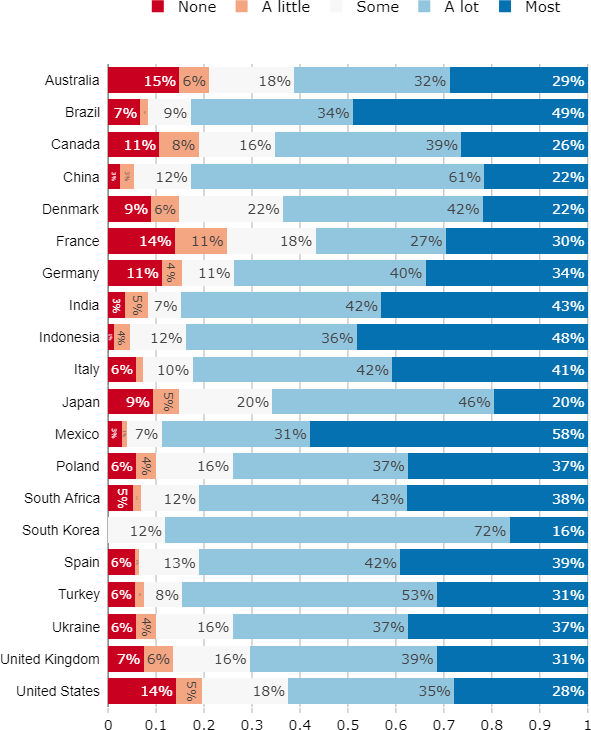
\includegraphics[height=.8\paperheight]{../figures/country_comparison/CC_anthropogenic_countries.png} 
	\end{figure}
\end{frame}

\begin{frame}{Limited understanding of climate science}%\addtocounter{framenumber}{-1}
	\begin{figure}%[h!]
	\centering
	\caption{Do you think that cutting global greenhouse gas emissions by half would be sufficient to eventually stop temperatures from rising? \\
	\footnotesize{\textit{Right answer: No}}} \vspace{-.5cm}
	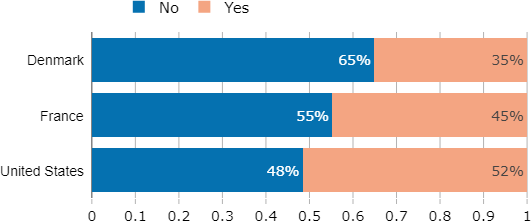
\includegraphics[height=.8\paperheight]{../figures/country_comparison/CC_dynamic_countries.png}
	
	\end{figure}
\end{frame}

\begin{frame}{Some mistakes on the factors of climate change}%\addtocounter{framenumber}{-1}
	\begin{figure}[h!]
	\centering
	\caption{Which of the following elements contribute to climate change? (Multiple answers are possible) \newline \footnotesize{\textit{Right answer: CO$_\text{2}$; Methane}}}
	\centering
	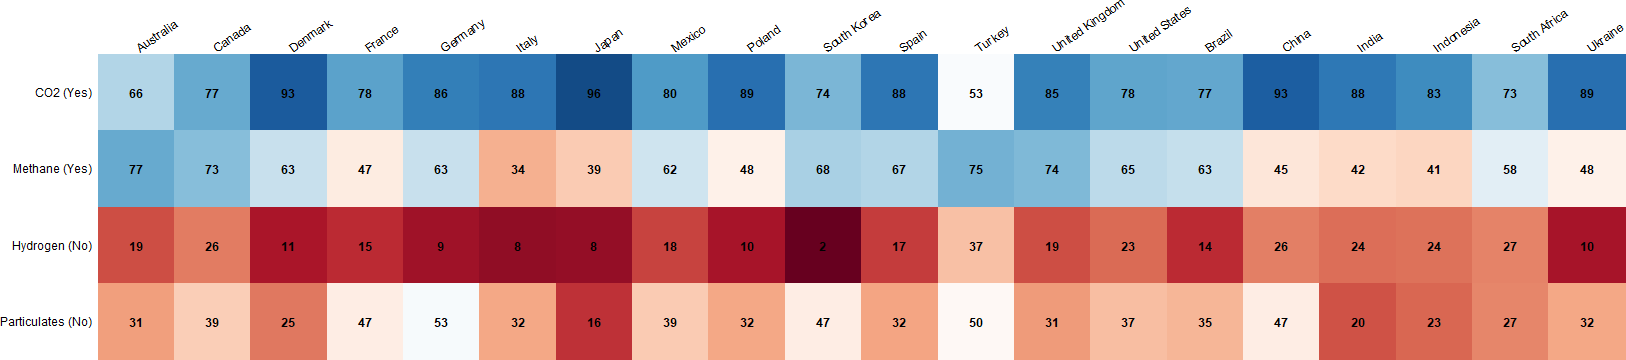
\includegraphics[width=\textwidth]{../figures/country_comparison/GHG_positive_countries.png}
	% \vspace{.2cm} \\
	% \includegraphics[height=.8\paperheight]{../figures/country_comparison/score_GHG_countries.png}
	
	% \textit{Score on GHG = CO$_\text{2}$ + methane + }not\textit{ hydrogen + }not\textit{ particulates}
	%\caption{Which of the following elements contribute to climate change? (Multiple answers are possible))}
	\end{figure}
\end{frame}
	
	% out
	% \begin{frame}{Climate change knowledge: GHG footprints}%\addtocounter{framenumber}{-1}
	% \begin{figure}[h!]
	% \centering
	% % \caption{Number of errors when ranking 3 items in terms of GHG emissions for three sectors}
	% \caption{Kendall tau distance to correct ranking of GHG footprints for three sectors ($\sim$ number of mistakes)}
	% \includegraphics[height=.8\paperheight]{../figures/country_comparison/scores_footprint_countries.png} \\
	% \centering
	% \caption{Rank the French/China/Western Europe/India in terms of GHG footprint}
	% \includegraphics[height=.8\paperheight]{../figures/country_comparison/score_footprint_regions_countries.png}
	% \vspace{.2cm}
	% % \\
	% % \small{Correct ranking: plane>car>coach, beef>chicken>pasta, coal>gas>wind/ US>Western Europe>China>India} \\
	% \end{figure}
	% \end{frame}
	
\begin{frame}{}%Climate change knowledge: Know relative emissions}
	\begin{figure}
	\caption{Which dish emits the most greenhouse gases? We consider that each dish weighs 200g.
	Please rank the items from 1 (most) to 3 (least).
	\footnotesize{\textit{Right answer: Beef (1), Chicken (2), Pasta (3)}}}
	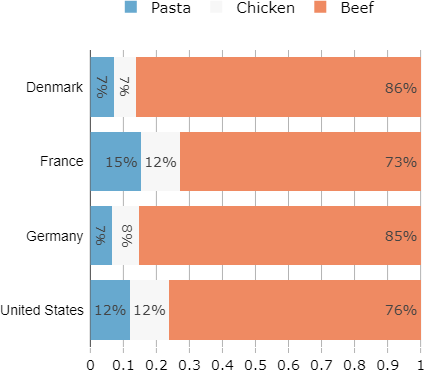
\includegraphics[height=.8\paperheight]{../figures/country_comparison/footprint_food_countries_most.png}
	\end{figure}
\end{frame}
	
\begin{frame}{}%Climate change knowledge: Know relative emissions}
	\begin{figure}
	\caption{If a [couple/family of 4] travels [distance] km from [City 1] to [City 2], with which mode of transportation do they emit the most greenhouse gases? 
	Please rank the items from 1 (most) to 3 (least).
	\newline \footnotesize{\textit{Right answer: Plane (1), Car (2), [Train/Coach] (3)}}} % TODO:other_countries Coach, towns
	\vspace{-.3cm}
	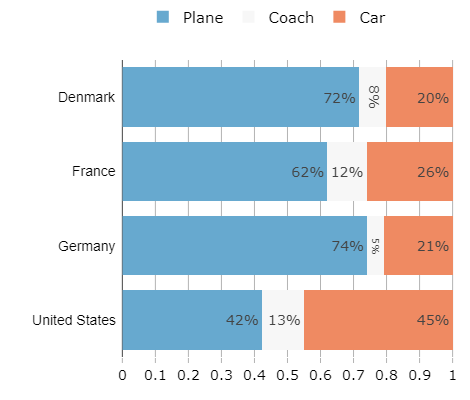
\includegraphics[height=.8\paperheight]{../figures/country_comparison/footprint_transport_countries_most.png}
	\end{figure}
\end{frame}
	
\begin{frame}{}%Climate change knowledge: Understand role of coal but misinformed about nuclear}%\addtocounter{framenumber}{-1}
	\begin{figure}
	\caption{Which source of electric energy emits the most greenhouse gases to provide power for a house?
	\newline \footnotesize{\textit{Right answer: Coal (1), Gas (2), Nuclear (3)}}}
	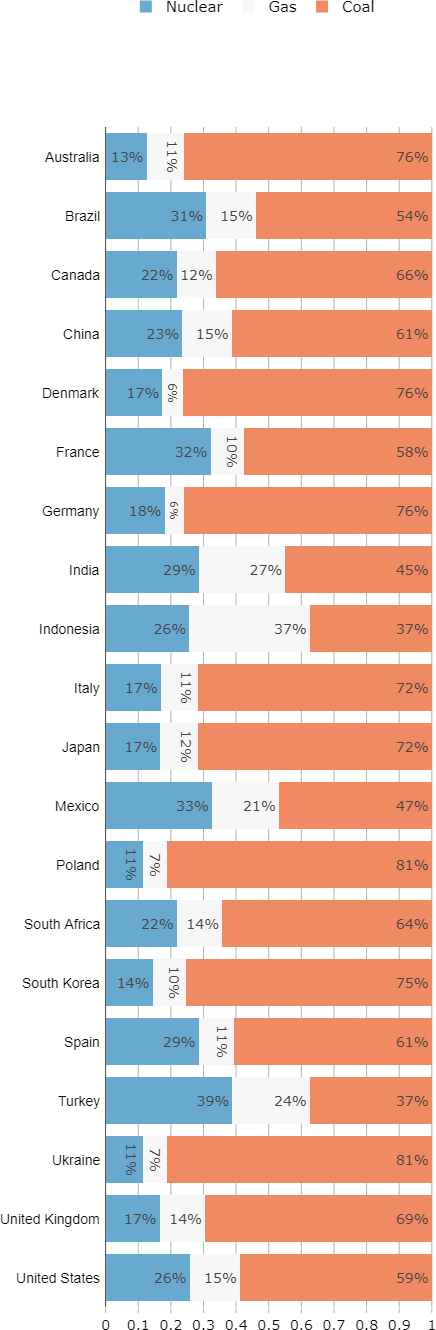
\includegraphics[height=.8\paperheight]{../figures/country_comparison/footprint_elec_countries_most.png}
	\end{figure}
	\end{frame}
	
	\begin{frame}{Correct understanding of total contributions}%\addtocounter{framenumber}{-1}
	\begin{figure}[h!]
	\centering
	\caption{Which region contributes most to global greenhouse gas emissions?
	\newline \footnotesize{\textit{Right answer: China (1), US (2), EU (3), India (4)}}} % True ranking: China>US>EU>India. 
	\vspace{-0.2cm}
	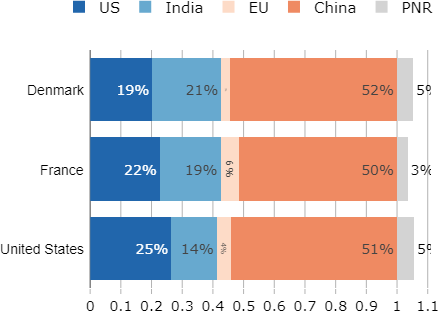
\includegraphics[height=.8\paperheight]{../figures/country_comparison/footprint_region_countries_most.png} % TODO!? least
	\end{figure}
\end{frame}
	
\begin{frame}{Poor understanding of per capita emissions}%\addtocounter{framenumber}{-1}
\begin{figure}[h!]
\centering
\caption{In which region does the consumption of an average person contribute most to climate change?
\newline \footnotesize{\textit{Right answer: US (1), EU (2), China (3), India (4)}}} % True ranking: US>EU>China>India. 
\vspace{-0.2cm}
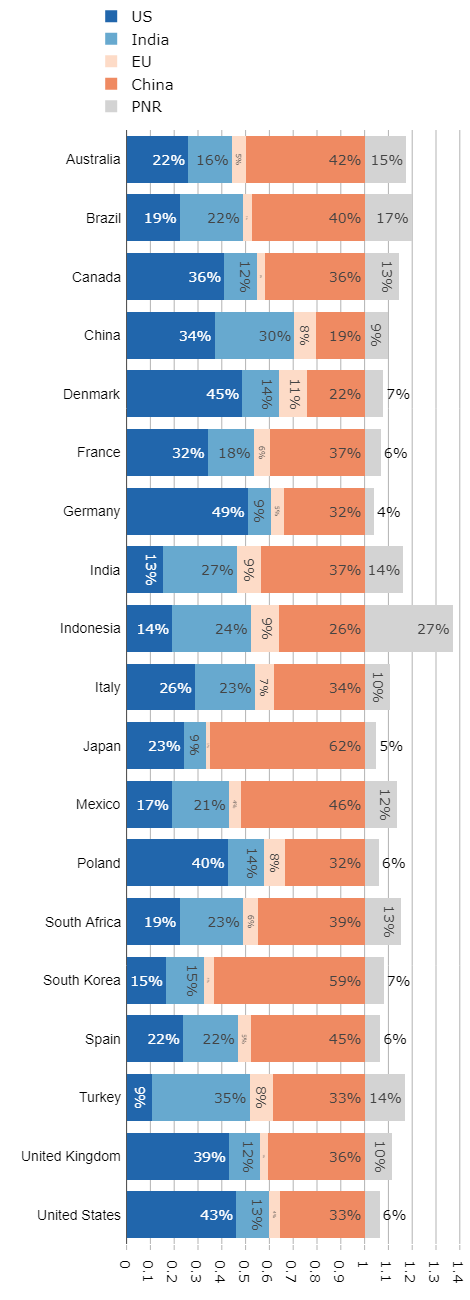
\includegraphics[height=.8\paperheight]{../figures/country_comparison/footprint_pc_countries_most.png}
\end{figure}
\end{frame}
	
\begin{frame}{Impacts of climate change: Credit a lot of effects}%\addtocounter{framenumber}{-1}
	\begin{figure}[h!]
	\centering
	%\caption{Impacts of climate change}
	%\vspace{2mm}
	\caption{If nothing is done to limit climate change, how likely do you think it is that climate change will lead to the following events?
	\newline\footnotesize{\textit{Right answer: Very likely: Severe droughts and heatwaves; Rising sea levels \\ \quad \quad \quad \quad \quad \quad Very unlikely: More frequent volcanic eruptions (No scientific certainty on the other items)}}}
	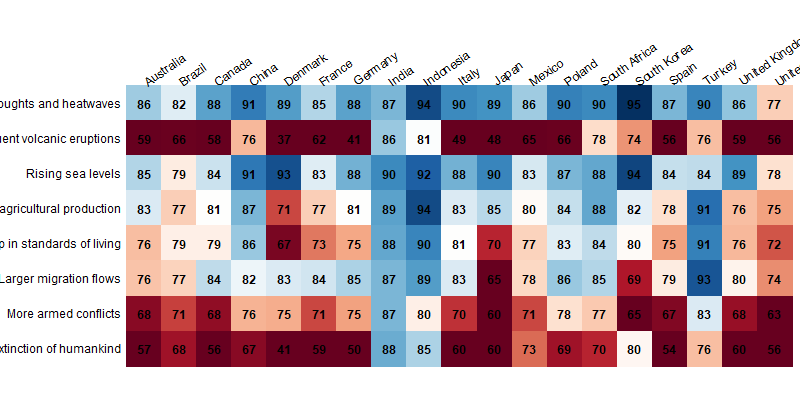
\includegraphics[width=\textwidth]{../figures/country_comparison/CC_impacts_positive_countries.png} \\
	%\caption{}
	\end{figure}
\end{frame}
	
\begin{frame}{Diverging views on whether net zero is feasible}%\addtocounter{framenumber}{-1}
	\begin{figure}[h!]
	\centering
	%\caption{Impacts of climate change}
	%\vspace{2mm}
	\caption{To what extent do you think that it is technically feasible to stop greenhouse gas emissions by the end of the century while sustaining satisfactory standards of living in [country]?}
	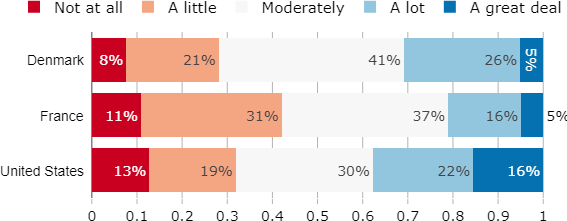
\includegraphics[height=.8\textheight]{../figures/country_comparison/net_zero_feasible_countries.png} \\
	%\caption{}
	\end{figure}
\end{frame}
	
\begin{frame}{Diverging views on whether net zero is feasible}%\addtocounter{framenumber}{-1}
	\begin{figure}[h!]
	\centering
	%\caption{Impacts of climate change}
	%\vspace{2mm}
	\caption{To what extent do you think that it is technically feasible to stop greenhouse gas emissions by the end of the century while sustaining satisfactory standards of living in [country]?}
	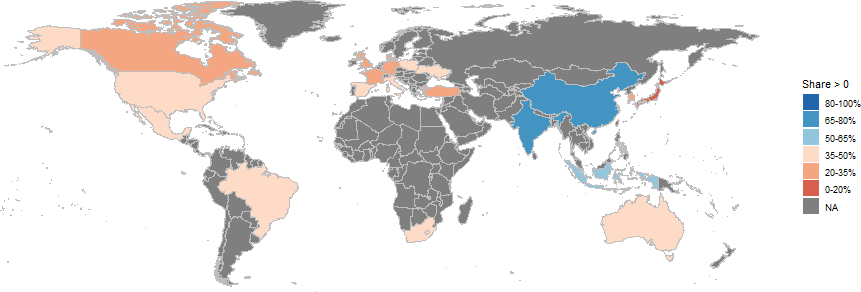
\includegraphics[width=\textwidth]{../figures/maps/net_zero_feasible.png} \\
	%\caption{}
	\end{figure}
\end{frame}
	
\begin{frame}{Diverging views on whether net zero is feasible}%\addtocounter{framenumber}{-1}
	\begin{figure}[h!]
	\centering
	%\caption{Impacts of climate change}
	%\vspace{2mm}
	\caption{To what extent do you think that it is technically feasible to stop greenhouse gas emissions by the end of the century while sustaining satisfactory standards of living in [country]?}
	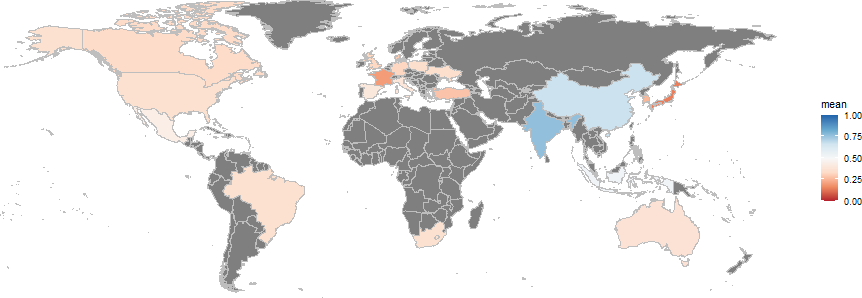
\includegraphics[width=\textwidth]{../figures/maps/net_zero_feasible_cont.png} \\
	%\caption{}
	\end{figure}
\end{frame}

\begin{frame}{Diverging views on whether net zero is feasible}%\addtocounter{framenumber}{-1}
	\begin{figure}[h!]
	\centering
	%\caption{Impacts of climate change}
	%\vspace{2mm}
	%\caption{To what extent do you think that it is technically feasible to stop greenhouse gas emissions by the end of the century while sustaining satisfactory standards of living in [country]?}
	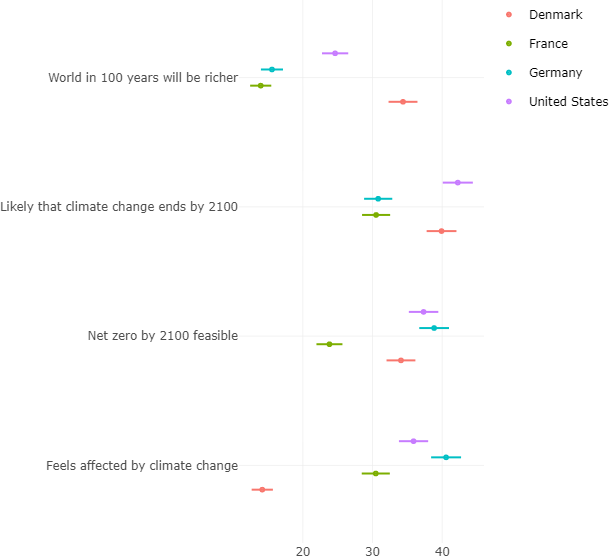
\includegraphics[height=.8\textheight]{../figures/country_comparison/future_by_country.png} \\
	%\caption{}
	\end{figure}
\end{frame}

\begin{frame}{Diverging views on whether net zero is feasible}%\addtocounter{framenumber}{-1}
	\begin{figure}[h!]
	\centering
	%\caption{Impacts of climate change}
	%\vspace{2mm}
	%\caption{To what extent do you think that it is technically feasible to stop greenhouse gas emissions by the end of the century while sustaining satisfactory standards of living in [country]?}
	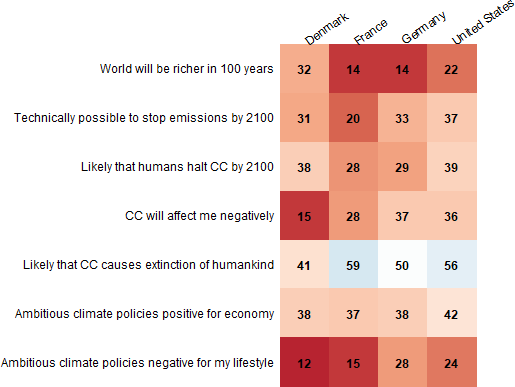
\includegraphics[width=\textwidth]{../figures/country_comparison/future_positive_countries.png} \\
	%\caption{}
	\end{figure}
\end{frame}

\section{(Mis)perceptions of climate policies}

\begin{frame}{Policies precisely described}%\addtocounter{framenumber}{-1}
	\begin{itemize}
	\ip \textcolor{blue}{Ban on Combustion Engine Cars}: To fight climate change, car producers can be required by law to produce cars that emit less CO$_\text{2}$ per km of the cars they sell. The emission limit is lowered every year so that only electric or hydrogen vehicles can be sold after 2030. This policy is called a \textit{ban on combustion-engine cars}.
	\ip \textcolor{blue}{Green Infrastructure Program}: A green infrastructure program is a large public investment program, which would be financed by additional public debt, to accomplish the transition needed to cut greenhouse gases emissions. Investments would concern renewable power plants, public transportation, thermal renovation of building, and sustainable agriculture.
	\ip \textcolor{blue}{Carbon Tax with Cash Transfers}: To fight climate change, the French government can make greenhouse gas emissions costly, to make people and firms change their equipment and reduce their emissions. The government could do this through a policy called a carbon tax with cash transfers. Under such a policy, the government would tax all products that emit greenhouse gas. For example, the price of gasoline would increase by 10 cents per liter. To compensate households for the price increases, the revenues from the carbon tax would be redistributed to all households, regardless of their income. Each adult would thus receive 160\euro{} per year.
	\end{itemize}
\end{frame}
	

\begin{frame}{Many think they would lose out}%\addtocounter{framenumber}{-1}
	\begin{figure}[h!]
	\centering
	\caption{%\textit{Comparison of responses to each policy question:} 
	Do you think that \textcolor{blue}{financially your household} would win or lose from \textit{the policy}?}
	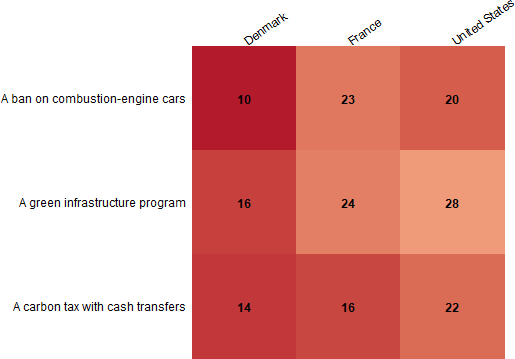
\includegraphics[width=\textwidth]{../figures/country_comparison/policies_win_lose_self_positive_countries.png}
	\vspace{-.1cm}
	\centering
	\caption{%\textit{Comparison of responses to each policy question:} 
	In your view, would those living in \textcolor{blue}{rural areas} win or lose from \textit{the following policy}?}
	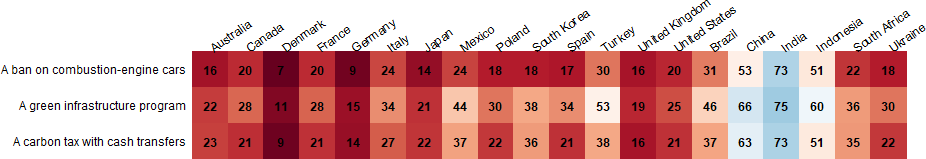
\includegraphics[width=\textwidth]{../figures/country_comparison/policies_win_lose_rural_positive_countries.png}
	%\caption{}
	\end{figure}
\end{frame}
	
\begin{frame}{Most view rich winning and poor losing}%\addtocounter{framenumber}{-1}
	\begin{figure}[h!]
	\centering
	\caption{%\textit{Comparison of responses to each policy question:} 
	In your view, would \textcolor{blue}{high-income} earners win or lose from \textit{the following policy}?}
	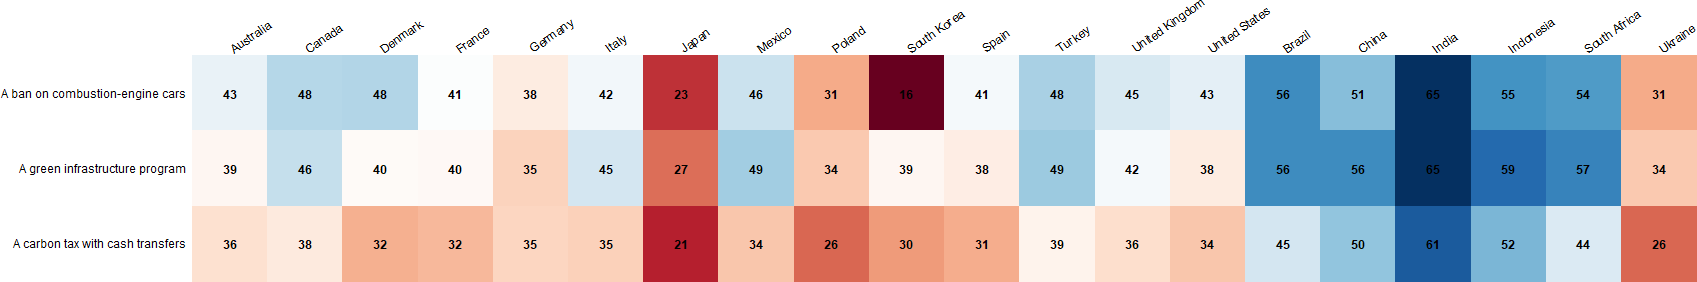
\includegraphics[width=\textwidth]{../figures/country_comparison/policies_win_lose_rich_positive_countries.png}
	\vspace{-.1cm}
	\centering
	\caption{%\textit{Comparison of responses to each policy question:} 
	In your view, would \textcolor{blue}{low-income} earners win or lose from \textit{the following policy}?}
	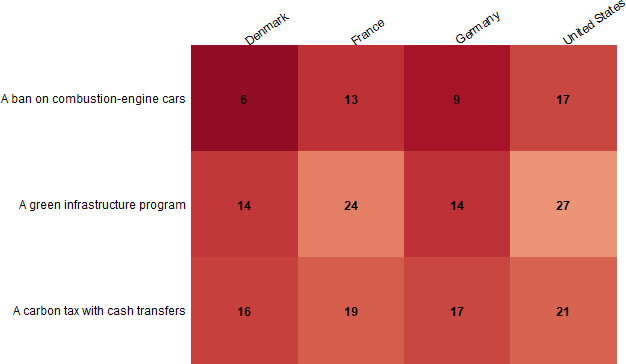
\includegraphics[width=\textwidth]{../figures/country_comparison/policies_win_lose_poor_positive_countries.png}
	%\caption{}
	\end{figure}
\end{frame}
	
\begin{frame}{See the middle class gains close to the poor's}%\addtocounter{framenumber}{-1}
	\begin{figure}[h!]
	\centering
	\caption{%\textit{Comparison of responses to each policy question:} 
	In your view, would the \textcolor{blue}{middle-class} win or lose from \textit{the following policy}?}
	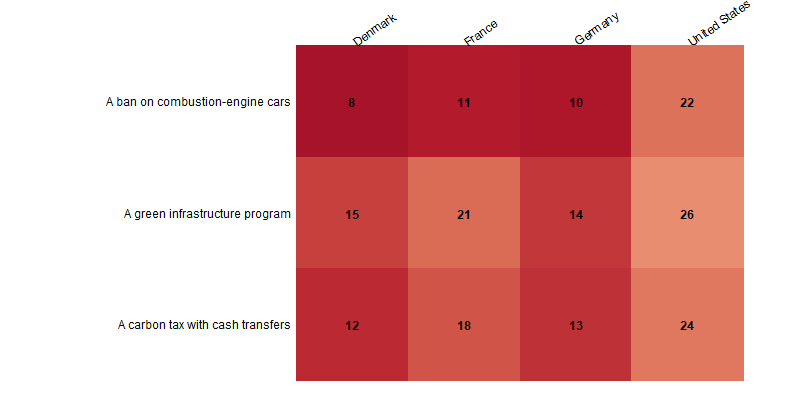
\includegraphics[width=\textwidth]{../figures/country_comparison/policies_win_lose_middle_positive_countries.png}
	%\caption{}
	\vspace{-.1cm}
	\centering
	\caption{%\textit{Comparison of responses to each policy question:} 
	In your view, would \textcolor{blue}{low-income} earners win or lose from \textit{the following policy}?}
	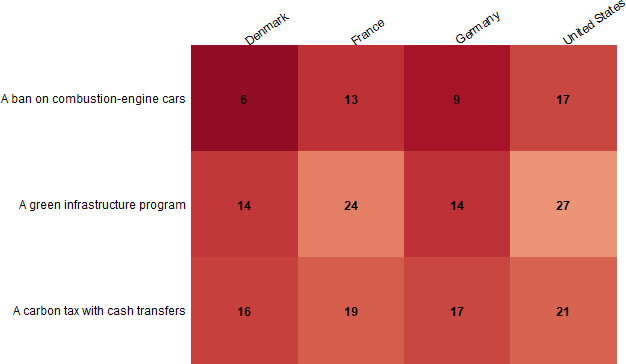
\includegraphics[width=\textwidth]{../figures/country_comparison/policies_win_lose_poor_positive_countries.png}
	%\caption{}
	\end{figure}
\end{frame}
	
% \begin{frame}{Only investments gather more positive than negative views}%\addtocounter{framenumber}{-1}
% 	\begin{figure}[h!]
% 	\centering
% 	\caption{%\textit{Comparison of responses to each policy question:} 
% 	Do you agree or disagree with the following statement? \textit{The policy} would have a \textcolor{blue}{\textbf{large} effect on the French economy and employment}.}
% 	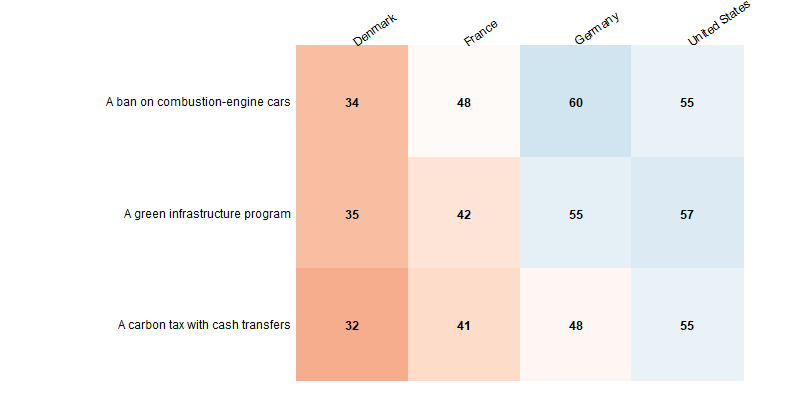
\includegraphics[width=\textwidth]{../figures/country_comparison/policies_large_effect_positive_countries.png}
% 	\vspace{-.1cm}
% 	\centering % TODO!
% 	\caption{%\textit{Comparison of responses to each policy question:} 
% 	Do you agree or disagree with the following statement? \textit{The policy} would have a \textcolor{blue}{\textbf{positive [or \textit{not} negative]} effect on the French economy and employment}.}
% 	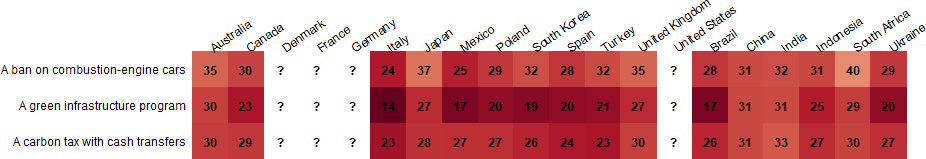
\includegraphics[width=\textwidth]{../figures/country_comparison/policies_positive_negative_positive_countries.png}
% 	\caption{}
% 	\end{figure}
% \end{frame}
	
\begin{frame}{Some acquiescence bias}%\addtocounter{framenumber}{-1}
	\begin{figure}[h!]
	\centering
	\caption{%\textit{Comparison of responses to each policy question:} 
	Do you agree or disagree with the following statement? \textit{The policy} would have a \textcolor{blue}{\textbf{positive} effect on the French economy and employment}.}
	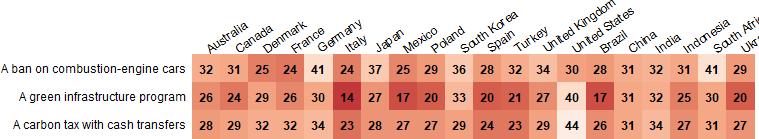
\includegraphics[width=.95\textwidth]{../figures/country_comparison/policies_positive_effect_positive_countries.png}
	\vspace{-.1cm}
	% \centering % TODO!
	% \caption{%\textit{Comparison of responses to each policy question:} 
	% Do you agree or disagree with the following statement? \textit{The policy} would have a \textcolor{blue}{\textbf{negative} effect on the French economy and employment}.}
	% 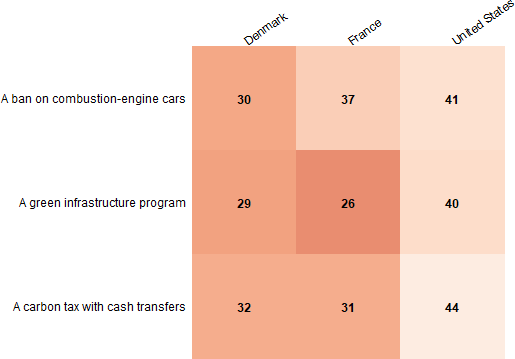
\includegraphics[width=\textwidth]{../figures/country_comparison/policies_negative_effect_positive_countries.png}
	% \caption{}
	\end{figure}
\end{frame}


% \begin{frame}{Policies seen as costly but effective}%
% 	%\addtocounter{framenumber}{-1}
	
% 	%\textbf{Problem:} strong acquiescence bias. In the pilot, 53-59\% agreed that it was ``cost-effective''. Formulation changed to ``costly'' and 56-57\% agree.
% 	\begin{figure}[h!]
% 	\vspace{-.1cm}
% 	\centering
% 	\caption{%\textit{Comparison of responses to each policy question:} 
% Do you agree or disagree with the following statement? \textit{The policy} would be \textcolor{blue}{costless [or \textit{not} costly] to fight climate change}} % TODO!
% 	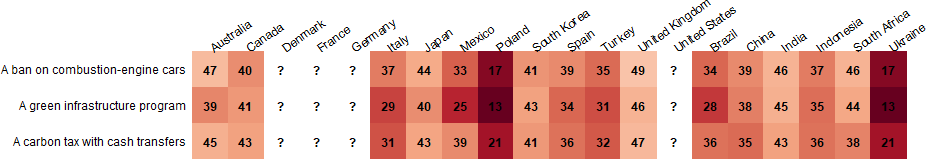
\includegraphics[width=\textwidth]{../figures/country_comparison/policies_costless_costly_positive_countries.png}
% 	% \caption{ \textcolor{blue}{would reduce air pollution}}
% 	% \includegraphics[width=\textwidth]{../figures/country_comparison/policies_less_pollution_positive_countries.png}
% 	%\caption{}
% 	\end{figure}
% \end{frame}
	
\begin{frame}{Incentives are acknowledged}
	\begin{figure}[h!]
	\vspace{-.1cm}
	\centering
	\caption{%\textit{Comparison of responses to each policy question:} 
Do you agree or disagree with the following statement? \textit{The policy} would ...} % TODO!
	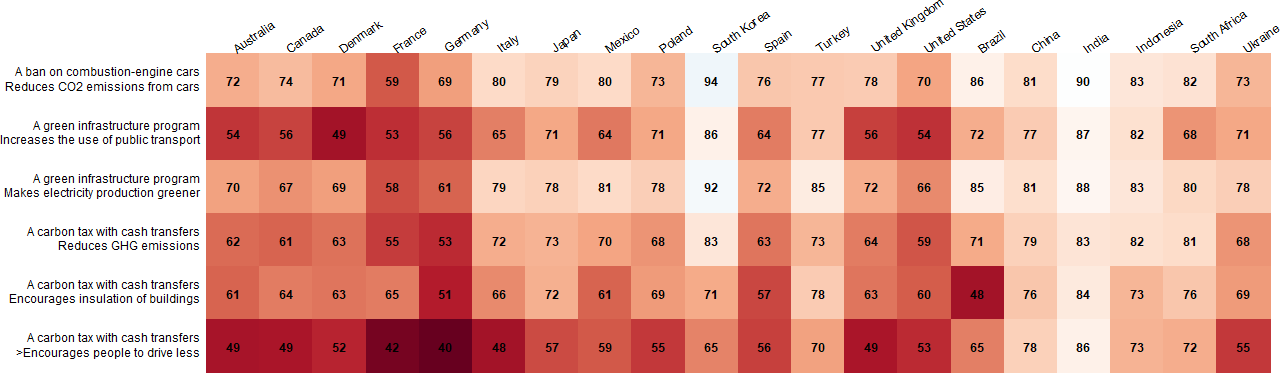
\includegraphics[width=\textwidth]{../figures/country_comparison/policies_effects_positive_countries.png}
	%\caption{}
	\end{figure}
\end{frame}
	
	
	% \begin{frame}{Fairness as main motive for support}%\addtocounter{framenumber}{-1}
	% \begin{figure}[h!]
	% \vspace{-.1cm}
	% \centering
	% \caption{%\textit{Comparison of responses to each policy question:} 
	%Do you agree or disagree with the following statement:"The \textit{policy} is \textcolor{blue}{fair}."}
	% \includegraphics[height=.8\paperheight]{../figures/country_comparison/policies_fair_countries.png}
	% \vspace{-.1cm}
	% \centering
	% \caption{%\textit{Comparison of responses to each policy question:} 
	%Do you \textcolor{blue}{support or oppose} \textit{the following policy}?}
	% \includegraphics[height=.8\paperheight]{../figures/country_comparison/policies_support_countries.png}
	% %\caption{}
	% \end{figure}

\begin{frame}{Carbon tax support higher when benefits are made salient}%\addtocounter{framenumber}{-1}
	\begin{figure}[h!]
	\centering
	\caption{Governments can use the revenues from carbon taxes in different ways. Would you support or oppose introducing a carbon tax that would raise gasoline prices by 10 centimes par litre, if the government used this revenue to finance...}
	\vspace{-.2cm}
	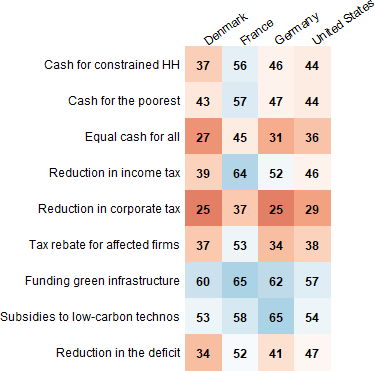
\includegraphics[width=\textwidth]{../figures/country_comparison/tax_positive_countries.png}
	%\caption{}
	\end{figure}
\end{frame}
		
			


\section{(Un)willingness to change behavior}
% 4) Can we show aversion to changing one’s own life style? Or lack of understanding of the magnitudes of what has to be done?
\begin{frame}{Willing to adopt the less restrictive behaviors}%\addtocounter{framenumber}{-1}
	\begin{figure}[h!]
	\centering
	\caption{Here are possible habits that experts say would help reduce greenhouse gas emissions.
	To what extent would you be willing to adopt the following behaviors?}
	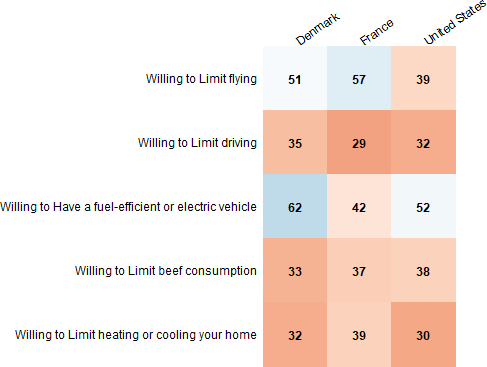
\includegraphics[width=\textwidth]{../figures/country_comparison/willing_positive_countries.png} \\
	\end{figure}
\end{frame}
	
\begin{frame}{Main factor needed to change lifestyle: fairness}%\addtocounter{framenumber}{-1}
	\begin{figure}[h!]
	\centering
	\caption{How important are the factors below in order for you to adopt a sustainable lifestyle (i.e. limit driving, flying, and consumption, cycle more, etc.)?}
	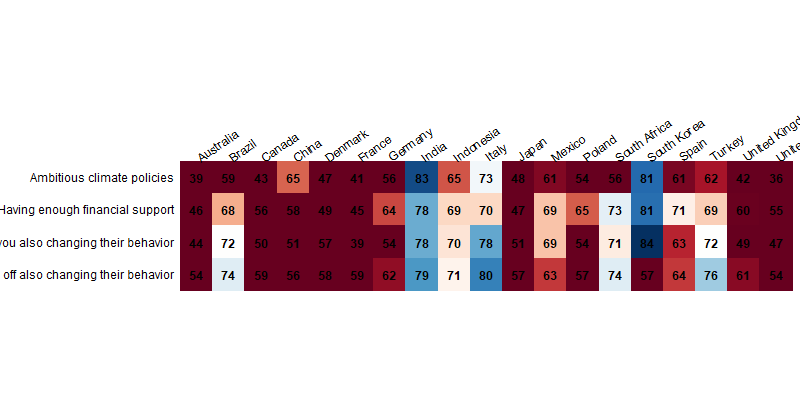
\includegraphics[width=\textwidth]{../figures/country_comparison/condition_positive_countries.png}
	\end{figure}
\end{frame}
	

\section{Effects of informational video treatments}
% TODO!

\begin{frame}{}%\addtocounter{framenumber}{-1}
	\begin{table}[h!]
	\caption{Attitudes towards Climate Change}
	\begin{center}
	\scalebox{.6}{
\begin{tabular}{@{\extracolsep{5pt}}lccccc} 
\\[-1.8ex]\hline 
\hline \\[-1.8ex] 
\\[-1.8ex] & CC caused by humans & CC likely to cause extinction & Donation (in \% of max) & FR should fight CC & Willing to limit driving \\ 
\hline \\[-1.8ex] 
 Control group mean & 0.567 & 0.587 & 24.924 & 0.778 & 0.321  \\ \hline \\[-1.8ex] Treatment: Climate & 0.096$^{***}$ & $-$0.034 & 2.490 & 0.006 & $-$0.020 \\ 
  & (0.029) & (0.031) & (1.694) & (0.026) & (0.029) \\ 
  & & & & & \\ 
 Treatment: Policy & 0.037 & $-$0.055$^{*}$ & $-$0.561 & $-$0.036 & $-$0.030 \\ 
  & (0.028) & (0.030) & (1.644) & (0.025) & (0.028) \\ 
  & & & & & \\ 
 Treatment: Both & 0.052$^{*}$ & $-$0.021 & $-$1.632 & $-$0.013 & 0.013 \\ 
  & (0.029) & (0.031) & (1.666) & (0.026) & (0.028) \\ 
  & & & & & \\ 
\hline \\[-1.8ex] 

Observations & 1,985 & 1,988 & 1,988 & 1,988 & 1,988 \\ 
\hline 
\hline \\[-1.8ex] 
\end{tabular} }
	\end{center} % TODO: why not 2006 obs.?
		{\tiny Note: The \textit{CC caused by humans} indicator variable equals one if the respondent thinks a lot or most of climate change is due to human actions. The \textit{CC likely to cause extinction} indicator variable equals one if the respondent thinks climate change is somewhat likely or very likely to cause the extinction of humankind if nothing is done to limit it. The \textit{Donation} variable is a continuous variable equal to the amount the respondent is willing to give to a charity. The \textit{should fight CC} indicator variable equals one if the respondent strongly agrees that their country ``should take measures to fight climate change''. The \textit{Willing to limit driving} indicator variable equals one if the respondent is willing a lot or a great deal to limit driving. The three \textit{treatment} indicator variables indicate difference in mean compared to the control group (people who did not see any video). Controls include socio-demographic, left-right leaning, last vote and whether the respondent's household was hit by the COVID-19 pandemic. Standard errors are in parentheses.  *p$<$0.1; **p$<$0.05; ***p$<$0.01}
	\end{table}
	\end{frame}
	
	\begin{frame}{}%\addtocounter{framenumber}{-1}
	\begin{table}[h!]
	\caption{Support for policies}
	\begin{center}
	\scalebox{.7}{
\begin{tabular}{@{\extracolsep{5pt}}lcccc} 
\\[-1.8ex]\hline 
\hline \\[-1.8ex] 
 & \multicolumn{4}{c}{Support} \\ 
\cline{2-5} 
\\[-1.8ex] & Carbon tax with transfers & Green Infrastructure Program & Ban on combustion-engine cars & Average over 3 policies \\ 
\hline \\[-1.8ex] 
 Control group mean & 0.282 & 0.582 & 0.274 & 0.444  \\ \hline \\[-1.8ex] Treatment: Climate & 0.061$^{**}$ & 0.037 & 0.032 & 0.035 \\ 
  & (0.030) & (0.030) & (0.029) & (0.031) \\ 
  & & & & \\ 
 Treatment: Policy & 0.079$^{***}$ & 0.033 & 0.061$^{**}$ & 0.051$^{*}$ \\ 
  & (0.029) & (0.029) & (0.028) & (0.030) \\ 
  & & & & \\ 
 Treatment: Both & 0.146$^{***}$ & 0.037 & 0.100$^{***}$ & 0.099$^{***}$ \\ 
  & (0.029) & (0.030) & (0.029) & (0.030) \\ 
  & & & & \\ 
\hline \\[-1.8ex] 

Observations & 1,988 & 1,988 & 1,988 & 1,988 \\ 
\hline 
\hline \\[-1.8ex] 
\end{tabular} }
	\end{center}
		{\footnotesize Note: The dependent variables are indicator variables equal to one if the respondent `Strongly supports'' or ``Somewhat supports'' the policy. The \textit{Average over 3 policies} takes the average of the respondent's answers for the three policies. It equals one if the respondent supports all three policies, 2/3 if she supports two, 1/3 if she supports only one, and 0 if she supports none. %See notes under previous Table for a description of the covariates.
		\newline Controls include socio-demographic, left-right leaning, last vote and whether the respondent's household was hit by the COVID-19 pandemic. Standard errors are in parentheses. *p$<$0.1; **p$<$0.05; ***p$<$0.01}
	\end{table}
	\end{frame}
	
	\begin{frame}{}%\addtocounter{framenumber}{-1}
	\begin{table}[h!]
	\caption{Attitudes towards policies}
	\begin{center}
	\scalebox{.7}{
\begin{tabular}{@{\extracolsep{5pt}}lccccc} 
\\[-1.8ex]\hline 
\hline \\[-1.8ex] 
\\[-1.8ex] & Fair & HH would win & Poor would win & Large economic effect & Negative economic effect \\ 
\hline \\[-1.8ex] 
 Control group mean & 0.436 & 0.292 & 0.173 & 0.592 & 0.41  \\ \hline \\[-1.8ex] Treatment: Climate & 0.011 & 0.040 & 0.014 & 0.013 & 0.007 \\ 
  & (0.030) & (0.029) & (0.026) & (0.030) & (0.031) \\ 
  & & & & & \\ 
 Treatment: Policy & 0.025 & 0.026 & 0.091$^{***}$ & 0.035 & 0.017 \\ 
  & (0.030) & (0.029) & (0.026) & (0.030) & (0.031) \\ 
  & & & & & \\ 
 Treatment: Both & 0.091$^{***}$ & 0.094$^{***}$ & 0.149$^{***}$ & 0.053$^{*}$ & 0.028 \\ 
  & (0.031) & (0.030) & (0.026) & (0.031) & (0.031) \\ 
  & & & & & \\ 
\hline \\[-1.8ex] 

Observations & 1,982 & 1,864 & 1,963 & 1,982 & 1,982 \\ 
\hline 
\hline \\[-1.8ex] 
\end{tabular} }
	\end{center}
		{\scriptsize Note: The dependent variables are discrete variables equal either to 0, 1/3, 2/3, or 1. They are equal to the average over the three policies mentioned in Table ``Support policies''. The \textit{Fair} variable equals one if the respondent strongly agrees or somewhat agrees that each of the three policies are fair. The \textit{HH/Poor would win} variables equal one if the respondent thinks her househould/the poorest would win a lot or mostly win from the three policies. The \textit{Large/Negative economic effect} variables equal one if the respondent strongly agrees or somewhat agrees that the three policies would have a large/negative impact on the French economy and employment. 
		\newline Controls include socio-demographic, left-right leaning, last vote and whether the respondent's household was hit by the COVID-19 pandemic. Standard errors are in parentheses. *p$<$0.1; **p$<$0.05; ***p$<$0.01}
	\end{table}
	\end{frame}

	
\section{Determinants of policy support (for France)} % TODO! other countries

\begin{frame}{}%\addtocounter{framenumber}{-1}
	\begin{figure}[h!]
	\caption{\% of positive responses by beliefs about climate change} % TODO! put CI on same line as they don't cross
	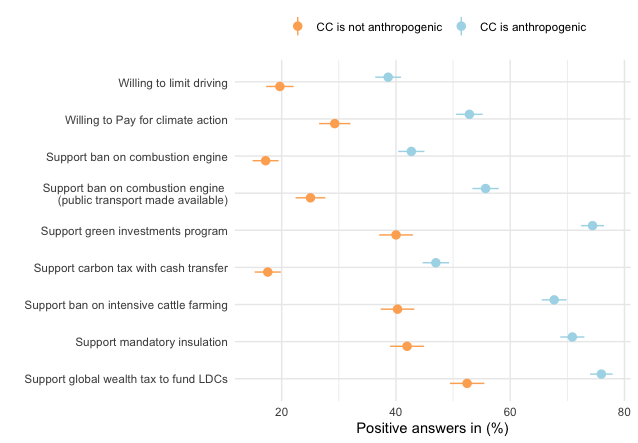
\includegraphics[width=.7\paperwidth]{../figures/FR/positive_all_by_CC_anthropogenic_FR.png} \\
	\end{figure}
	\end{frame}
	
	\begin{frame}{}%\addtocounter{framenumber}{-1}
	\begin{figure}[h!]
	\caption{\% of positive responses by trust in government}
	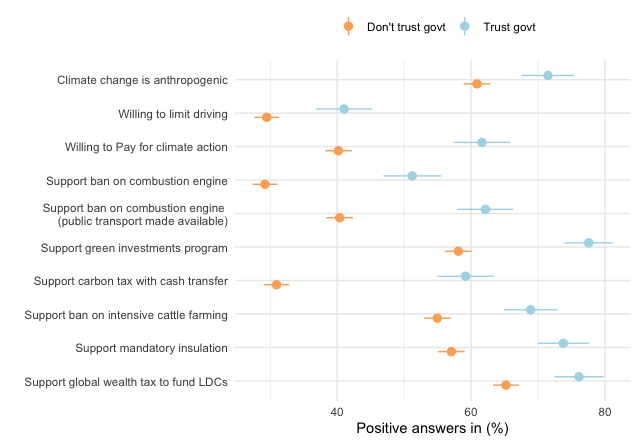
\includegraphics[width=.7\paperwidth]{../figures/FR/positive_all_by_trust_govt_FR.png} \\
	\end{figure}
	\end{frame}
	
	\begin{frame}{}%\addtocounter{framenumber}{-1}
	\begin{figure}[h!]
	\caption{\% of positive responses by living with child(ren) below 14}
	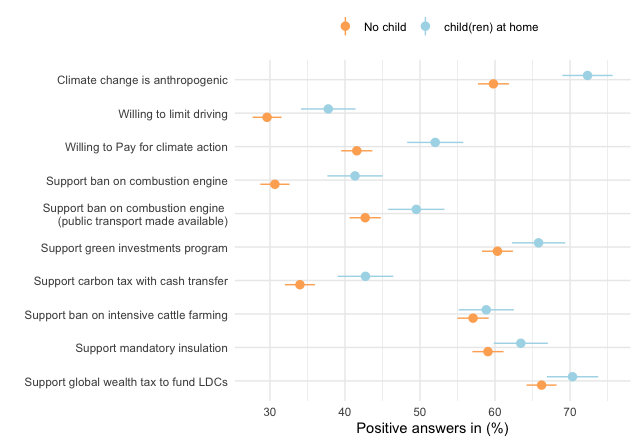
\includegraphics[width=.7\paperwidth]{../figures/FR/positive_all_by_children_FR.png} \\
	\end{figure}
	\end{frame}
	
	\begin{frame}{}%\addtocounter{framenumber}{-1}
	\begin{figure}[h!]
	\caption{\% of positive responses by age}
	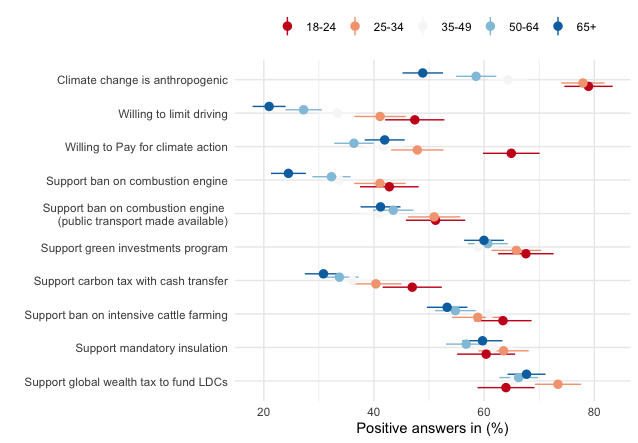
\includegraphics[width=.7\paperwidth]{../figures/FR/positive_all_by_age_FR.png} \\
	\end{figure}
	\end{frame}
	
	\begin{frame}{}%\addtocounter{framenumber}{-1}
	\begin{figure}[h!]
	\caption{\% of positive responses by diploma}
	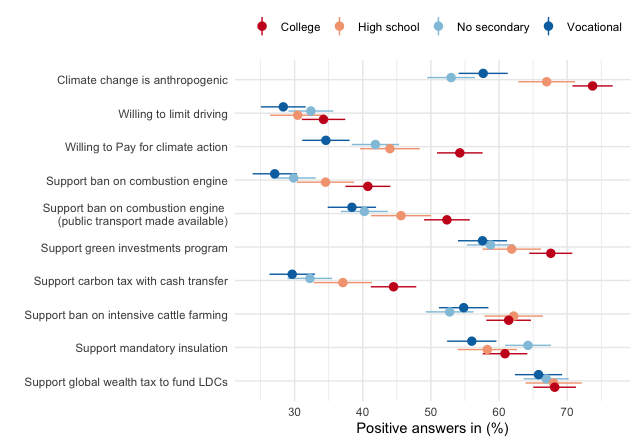
\includegraphics[width=.7\paperwidth]{../figures/FR/positive_all_by_diploma_FR.png} \\
	\end{figure}
	\end{frame}
	
	\begin{frame}{}%\addtocounter{framenumber}{-1}
	\begin{figure}[h!]
	\caption{\% of positive responses by working sector}
	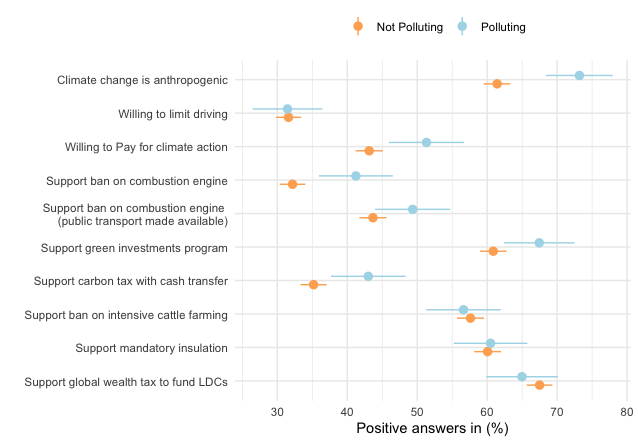
\includegraphics[width=.7\paperwidth]{../figures/FR/positive_all_by_polluting_sector_FR.png} \\
	\end{figure}
	\end{frame}
	
	\begin{frame}{}%\addtocounter{framenumber}{-1}
	\begin{figure}[h!]
	\caption{\% of positive responses by avalaibility of public transport}
	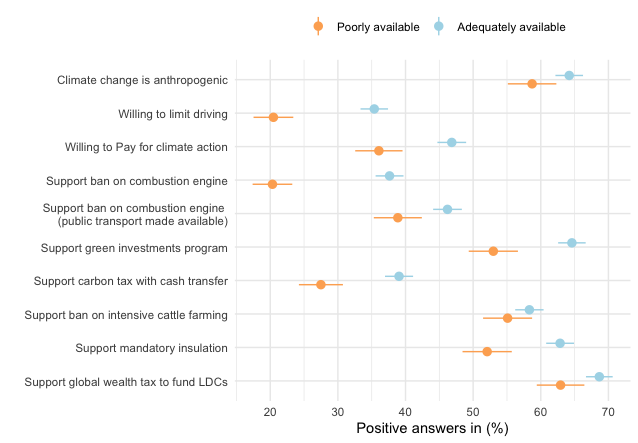
\includegraphics[width=.7\paperwidth]{../figures/FR/positive_all_by_availability_transport_FR.png} \\
	\end{figure}
	\end{frame}
	
	\begin{frame}{}%\addtocounter{framenumber}{-1}
	\begin{figure}[h!]
	\caption{\% of positive responses by urban category}
	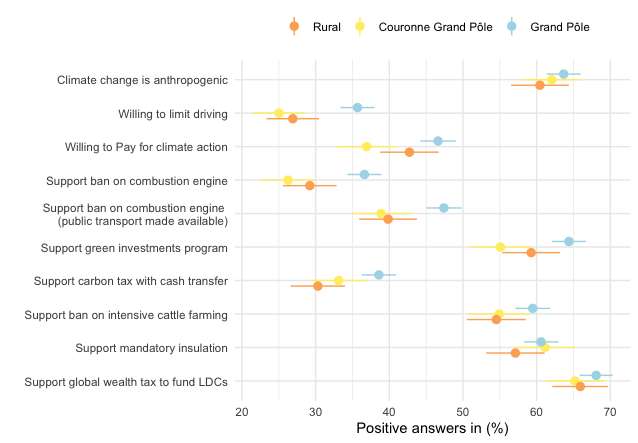
\includegraphics[width=.7\paperwidth]{../figures/FR/positive_all_by_urban_FR.png} \\
	\end{figure}
	\end{frame}
	
	\begin{frame}{}%\addtocounter{framenumber}{-1}
	\begin{figure}[h!]
	\caption{\% of positive responses by income}
	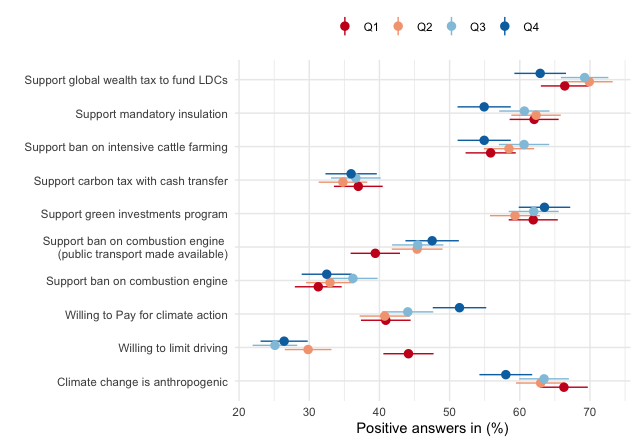
\includegraphics[width=.7\paperwidth]{../figures/FR/positive_all_by_income_FR.png} \\
	\end{figure}
	\end{frame}
	
	\begin{frame}{}%\addtocounter{framenumber}{-1}
	\begin{figure}[h!]
	\caption{\% of positive responses by support for the Yellow Vests}
	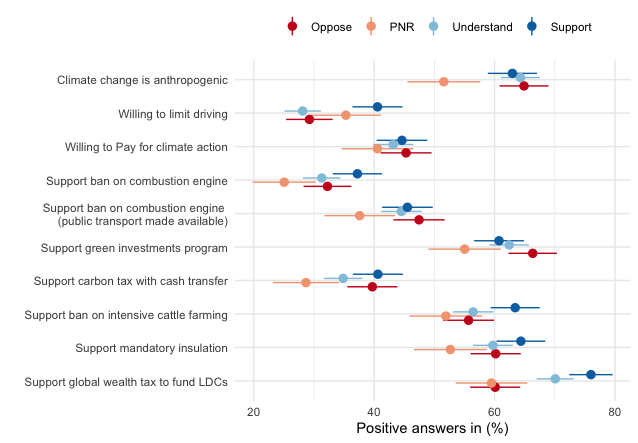
\includegraphics[width=.7\paperwidth]{../figures/FR/positive_all_by_yellow_vests_FR.png} \\
	\end{figure}
	\end{frame}
	
	\begin{frame}{}%\addtocounter{framenumber}{-1}
	\begin{figure}[h!]
	\caption{\% of positive responses by vote}
	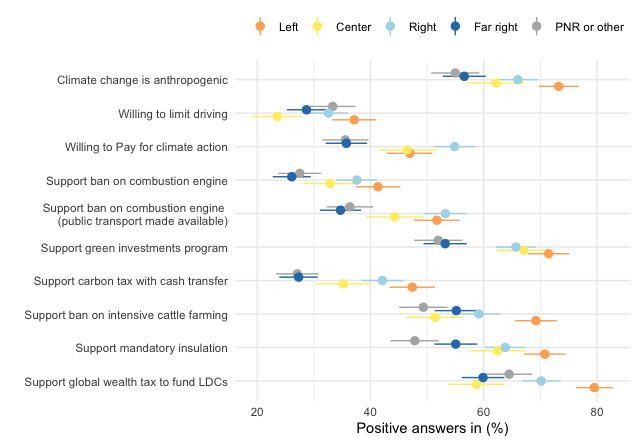
\includegraphics[width=.7\paperwidth]{../figures/FR/positive_all_by_vote_agg_FR.png} \\
	\end{figure}
	\end{frame}
	
	\begin{frame}{}%\addtocounter{framenumber}{-1}
	\begin{figure}[h!]
	\caption{\% of positive responses by gas expenses}
	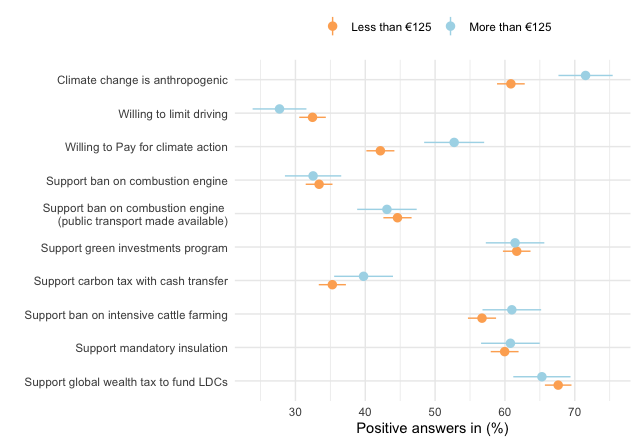
\includegraphics[width=.7\paperwidth]{../figures/FR/positive_all_by_gas_expenses_FR.png} \\
	\end{figure}
	\end{frame}
	
	% \begin{frame}{}%\addtocounter{framenumber}{-1}
	% \begin{figure}[h!]
	% \caption{\% of positive responses by heating expenses}
	% \includegraphics[height=.8\paperheight]{../figures/country_comparison/positive_all_by_heating_expenses_countries.png} \\
	% \end{figure}
	% \end{frame}
	
	% \begin{frame}{}%\addtocounter{framenumber}{-1}
	% \begin{figure}[h!]
	% \caption{Support for all policies -- Regression results}
	% \includegraphics[height=.8\paperheight]{../figures/country_comparison/coef_support_indices_countries.png} \\
	% \tiny{Note: Variables used in the analysis but not displayed:  origin, gender, and income. The policy support for all variable is an indicator variable equal to one if on average among the three policies the respondent somewhat or strongly support the policies (i.e., it is a dummy that the average support across policies is positive).}
	% \end{figure}
	% \end{frame}

\end{document}